\chapter{Design Specification}
This section includes the original design specification written in the third and fourth weeks of the project. It's second draft is shown here.

%==============================================================================
\section{Introduction}
%==============================================================================
The purpose of this document is to consider the project as an entire working system, and then break down the detailed aspects into easily manageable sections. The requirements will be transformed into the necessary data and client side structure, facilitating the creation a working application.

%==============================================================================
\section{Game Applications}
%==============================================================================
This design outlines two applications necessary for this project. Using two applications separates game logic and data persistence from user interaction and interface desgin.

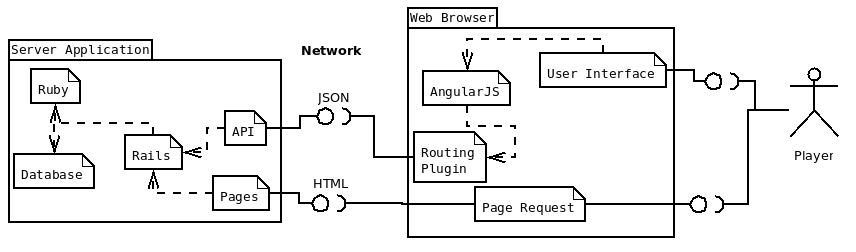
\includegraphics[width=\textwidth]{Images/app3/applications}

\subsection{The Server Side}
The server side application includes data persistence and the logic necessary to constrain user actions. The second is the client side application. Using a RESTful API provided by the server, this will represent the list of possible resources and actions as a Single Page Application (SPA), making it easy for users to make game choices and see the game react.

\subsection{Interoperability}
A RESTful API was chosen to improve interoperability, making the game deployable on various client side devices. This project will focus on a web-application, to be rendered in a web browser. However, once in place, native applications or other client side implementations could be created to render the game on a host of various devices.

In accordance with a RESTful API, resources will be represented with unique URIs. HTTP actions will be used to access, update or delete the data. JSON will be the default language to send data between the server and client.

\subsection{The Client Side}
The client side application will use data from the server to represent a game board and controls to the user. When users are authenticated by the system their actions will update resources on the server that relate to their account and games they are involved in. So data will be retrieved from the server, and occasionally updated by the client.

%==============================================================================
\section{Database Structure}
\subsection{Main Database Structure}
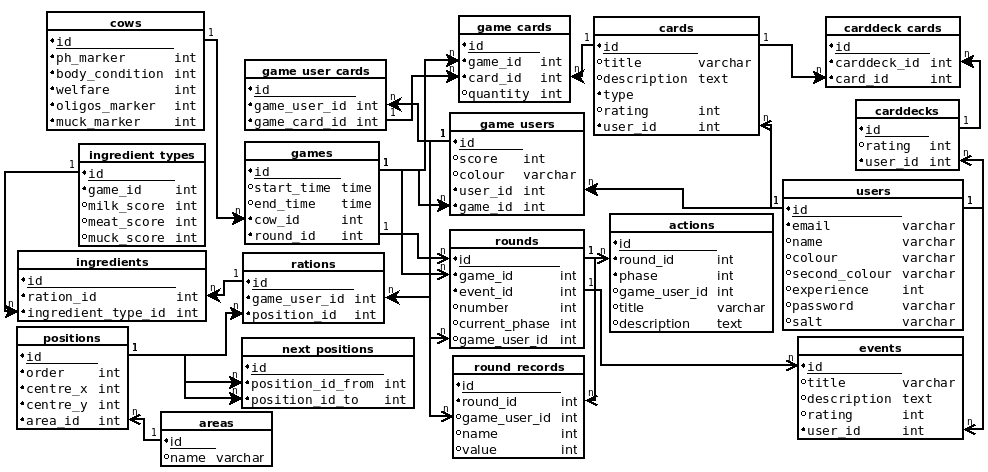
\includegraphics[width=\textwidth]{Images/app3/full-database}

\subsubsection{Conventions}
This design matches the Ruby On Rails Active Record convention. Tables names are plurals of the objects they contain. Primary keys are simply named 'id', and foreign keys are singular items \cite{ActiveRecordConvention}.

\subsubsection{Tables}
\paragraph{users} The \textbf{users} table stores details of players which allow them to login and store a few personal details. Their email, password and salt are to do with validation. Once logged in, players will be referred to by their name, and sometimes game pieces will be identified by a colour. The second colour is used in case two players in the same game have the same colour. A \textbf{users} experience will increase the more games they play.

\paragraph{game\_users} This is a table to join games with players in a many-to-many relationship. So it can be thought of as details that refer to a player and are specific to a game. A score and the determined colour (out of two possible) are needed per game the player is involved in.

\paragraph{games} One record is kept in this table for each \textbf{game} that is played. A start time and end time is recorded, and a reference to information in the \textbf{cow} table and the current round.

\paragraph{cow} The \textbf{cows} table shares a one-to-one relationship with the \textbf{games} table, only one cow is needed per game. Here values are recorded to persist the current value of markers which tell players what the state of health of the cow is in their game.

\paragraph{rounds} Rounds must be recorded, as when the game is created, the number of rounds is determined, and an event chosen for each round. So rounds identify themselves to a game, they have a number which indicates the order they appear in. The current phase is a number from one to four, relating to the possible phases. The active player is also recorded, if applicable. When the round is in the last phase, no player is active. Rounds have an event assigned when they are created, at the start of a game.

\paragraph{actions} These are created as the game progresses. They provide a record of what has happened in a round, used in the final review phase. The round and phase is necessary in an action, where as an action may be performed by a player, or may not. An example of an action is title: 'Made a ration', game\_user: 'player1', and description: 'Spent a water and energy to make a ration'. They are designed to be human readable, rather than machine readable.

\paragraph{round\_records} This table exists in order to record values, such as player's scores, from round to round. The 'name' field can be 'score' or 'cards', and the value indicates the number. This table is used for review and game statistics only.

\paragraph{rations} Each \textbf{game\_user} can have up to four rations. These are capsules for ingredients that have a set position, which can be updated by the owner in the movement phase.

\paragraph{positions} This table is necessary in order to tie the rations to the abstract shape of the game board. Positions are pre-set, and a single list is used for all games. Each position has an x and y position, which identifies where it will appear on the game board. It also has three images to represent it's shape. These are so that the area on the board can light up different colours depending if a player can move their ration to the position or not. Finally positions have an area and an order. This is so that the leading or rear ration can be determined. The leading ration is the one with the greatest area, and then the greatest order within that area.

\paragraph{next\_positions} This table defines a graph of positions. Positions can be considered nodes, and the next\_position records can be considered to be one-directional connections. So having a position it is possible to look up all the positions that lead to it, and all the positions that lead from it. This will confine where a user is allowed to move their rations. In the rumen, bi-directional connections are allowed, so two records will be needed to join neighbours.

\paragraph{areas} These correspond to the areas of the board: trough, oesophagus, rumen and intestines. They help order positions.

\paragraph{ingredients and ingredient\_types} A ration can have up to four ingredients. They are created by using cards with the corresponding ingredient, however, an ingredient record is only created when a ration is. Ingredient types store data about the number of points scored for each ingredient, as these are subject to change.

\paragraph{cards} These are all possible cards, for all possible games. Each card includes a title (eg: Medicine), a description (eg: Cow welfare +1), a rating which can be given by people who finish playing a game with that card, and the creator of the card is automatically assigned.

Another diagram exists describing the possibility of cards performing automatic effects, defined by users when they are created. But that may be implemented in a later phase, and so has been left out of this diagram for simplicity.

\paragraph{card\_decks and card\_deck\_cards} These tables organise the cards into decks, creating a many-to-many relationship between the \textbf{cards} table and the \textbf{card\_decks} table. When creating a game, a user can choose an existing card deck, or create a new one. To do this they choose the cards they want to include as well as the quantity of that card. The quantity defines how likely the card is to come from the deck, if card A has a quantity of 1, and card B a quantity of 4, card B is four times as likely as card 1, as with a real deck of cards. Card decks have a rating by those who have played a game using it.

\paragraph{game\_cards} As described above, a user chooses a deck of cards when creating a game. Because a deck could be edited by it's creator, these decks are copied to several other records, which define the unchangeable cards and quantities that will be used during the game.

\paragraph{game\_user\_cards} Within a game, a player accumulates a hand of cards. This table records this information by providing a many-to-many relationship between the \textbf{game\_users} and \textbf{game\_cards} tables.

\paragraph{events} Possible events that can happen in a game are stored in this table. The event has a title, description, rating and image. All describe the event.

\paragraph{round\_events} When a game is created it's number of rounds is determined, and an event given to each round. This table joins the rounds to events.

\subsection{Extra Database Structure}
If the project reaches the final phase, it will be necessary for cards and events to be created with automatically assignable actions that get carried out during games. To make that possible, the following database structure must be added to the existing one above.

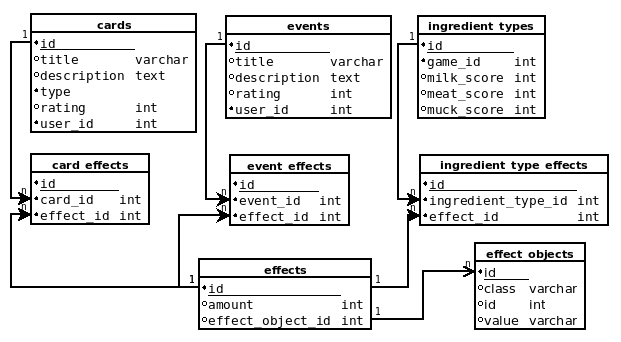
\includegraphics[width=\textwidth]{Images/app3/extra-database}

The \textbf{cards}, \textbf{events} and \textbf{ingredient\_types} tables are from the existing database. They each have a sub table which links certain instances of cards, events and ingredient types to the \textbf{effects} table. An effect is something that happens to another object in the database. The class field indicates which table that object is in, the id field picks out the row to effect, and the value says what the new, or relative value of the row should be.

An effect engine will need to be put in place to carry out these operations, but given this structure it should not be complicated to perform. If other effects are needed later, such as creating or removing an instance, they can be added as other tables that are linked to the \textbf{effects} table.

%==============================================================================
\section{RESTful API}
This section describes how the data in the previous section will be accessed via the server API. A strict standard of a RESTful API has been chosen in order to increase the organisation of interoperability between the server and client. The notation '[id]' has been used to represent a number that can be used to represent a resource.

\subsection{HTTP Operations}
Unless stated otherwise below, the HTTP operations used for URIs will follow the pattern described in this section.
\subsubsection{/resources}
This will return a collection of all the resources with the name 'resources', if the user has permission to access them. The following HTTP operations are allowed for this URI:
\begin{itemize}
	\item \textbf{POST} - creates a new 'resource'.
	\item \textbf{GET} - returns a list of all instances of 'resource'.
\end{itemize}
\subsubsection{/resources/[id]}
This will deal with a specific resource with the given id, if the user has permission to access it. The following HTTP operations are allowed for this URI:
\begin{itemize}
	\item \textbf{GET} - returns a single resource's details.
	\item \textbf{PUT} - replaces a resource's details.
	\item \textbf{PATCH} - updates part of a resource's details.
	\item \textbf{DELETE} - removes a resource.
\end{itemize}
\subsubsection{/resources/[id]/otherresources}
This will return a collection of all the resources with the name 'otherresources' that are related to the specific 'resource' identified by the id. This is only allowed if the user has permission to access them. The following HTTP operations are allowed for this URI:
\begin{itemize}
	\item \textbf{POST} - creates a new 'otherresource', but fills in the relation to the parent 'resource' automatically.
	\item \textbf{GET} - returns the 'otherresources' that are related to the 'resource', eg: are owned or created by it.
\end{itemize}
The same is true for further nested resources.
\subsubsection{/resources/[id]/otherresources/[id]}
This will deal with a specific resource with the given id, if the user has permission to access it. The following HTTP operations are allowed for this URI:
\begin{itemize}
	\item \textbf{GET} - returns a single resource's details. Resources at this level are read-only. To update or delete the resource, it can be accessed via it's base URI \textbf{/otherresources/[id]}.
\end{itemize}

\subsection{HTTP Data Types}
The API is designed to provide a service for a client. It should be possible to play a game by giving the correct values to the API without a client. However, this is not the intended use, therefore the default data type of the application will be JSON format. This is all that will be implemented for the core functionality.

When the game is fully functional, there is a chance it will be used with other clients that may demand XML or HTML data. Ruby on Rails makes it easy to return different data types, based on the requested file type. These data types can therefore be offered at a later stage.

For addressability, as far as possible resources will provide links to related resources dynamically in the data that is sent to the client.

\subsection{Resources}
\subsubsection{Users}
\begin{itemize}
	\item \textbf{/users} - a list of users.
	\item \textbf{/users/[id]} - a specific user.
	\item \textbf{/users/[id]/games} - games related to a specific user.
	\item \textbf{/users/[id]/games/[id]} - a specific game related to a specific user.
\end{itemize}
\subsubsection{Games}
\begin{itemize}
	\item \textbf{/games} - a list of games.
	\item \textbf{/games/[id]} - a specific game.
	\item \textbf{/games/[id]/cow} - a cow that is related to this game. It is a singleton.
	\item \textbf{/cows} - a list of all cow details, should you wish to know it.
	\item \textbf{/cows/[id]} - a specific cow's details, without going through the game.
	\item \textbf{/games/[id]/cards} - cards used within a game.
	\item \textbf{/games/[id]/users} - players of a game.
	\item \textbf{/games/[id]/users/[id]} - a specific player of a game.
	\item \textbf{/games/[id]/users/[id]/cards} - a list of cards belonging to a player.
	\item \textbf{/games/[id]/users/[id]/cards/[id]} - a specific card belonging to a player.
	\item \textbf{/games/[id]/users/[id]/rations} - a list of rations belonging to a player.
	\item \textbf{/games/[id]/users/[id]/rations/[id]} - a specific ration belonging to a player.
	\item \textbf{/games/[id]/users/[id]/rations/[id]/ingredients} - a list of ingredients in a specific ration belonging to a player.
	\item \textbf{/games/[id]/users/[id]/rations/[id]/ingredients/[id]} - a specific ingredient in a ration belonging to a player.
	\item \textbf{/games/[id]/round} - the current round in a game.
	\item \textbf{/games/[id]/rounds} - the current and previous rounds in a game, unless the user has permission to see all the rounds in a game.
	\item \textbf{/games/[id]/rounds/[id]} - a specific round in a game.
	\item \textbf{/games/[id]/rounds/[id]/actions} - a list of the actions that have happened in a round.
	\item \textbf{/games/[id]/rounds/[id]/actions/[id]} - a specific action within a round in a game.
	\item \textbf{/games/[id]/rounds/[id]/event} - the event that happened in a round. It is a singleton.
\end{itemize}

\subsubsection{Cards}
\begin{itemize}
	\item \textbf{/cards} - a list of all cards.
	\item \textbf{/cards/[id]} - a specific card.
	\item \textbf{/users/[id]/cards} - a list of cards the player has created.
	\item \textbf{/users/[id]/cards[id]} - a specific card that a player has created.
	\item \textbf{/decks} - a list of all decks.
	\item \textbf{/decks/[id]} - a specific deck of cards.
	\item \textbf{/decks/[id]/cards} - a list of all cards in a deck.
	\item \textbf{/decks/[id]/cards/[id]} - a specific card in a deck.
	\item \textbf{/users/[id]/decks} - a list of decks the player has created.
	\item \textbf{/users/[id]/decks[id]} - a specific deck that a player has created.
\end{itemize}

\subsubsection{Rounds and Events}
\begin{itemize}
	\item \textbf{/rounds} - a list of all the rounds. Rounds are not created by the client, so are read only.
	\item \textbf{/rounds/[id]} - a specific round.
	\item \textbf{/actions} - a list of all the actions.
	\item \textbf{/action/[id]} - a specific action.
	\item \textbf{/rounds/[id]/actions} - a list of actions that happened within a round.
	\item \textbf{/events} - a list of events.
	\item \textbf{/events/[id]} - a specific event.
	\item \textbf{/rounds/[id]/event} - the event that happened in a round. It is a singleton, and is read only.
	\item \textbf{/users/[id]/events} - a list of events created by this user.
	\item \textbf{/users/[id]/events/[id]} - a specific event created by this user.
\end{itemize}

\subsubsection{Positions and Areas}
Positions and areas are read only. They are the same for all games. Rations are updated with positions.
\begin{itemize}
	\item \textbf{/positions} - returns a list of all positions, in order.
	\item \textbf{/positions/[id]} - a single position's details.
	\item \textbf{/positions/[id]/next}  - a list of all positions from this position.
	\item \textbf{/positions/[id]/previous} - a list of all positions going to this position.
	\item \textbf{/areas} - a list of all areas, in order.
	\item \textbf{/areas/[id]} - a single area's details.
	\item \textbf{/areas/[id]/positions} - a list of positions in this area, in order.
	\item \textbf{/positions/[id]/graph/[number]} - uses the positions like a graph. A number must be supplied. The result will be a recursive list of positions, each with an array of their next positions. The depth is the number supplied.
\end{itemize}

%==============================================================================
\section{Client Structure}

\subsection{Pages}
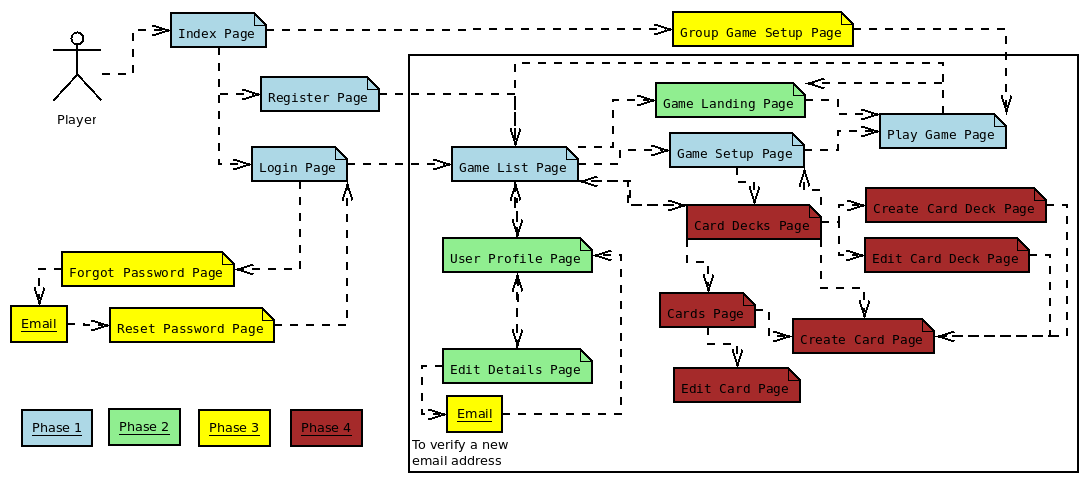
\includegraphics[width=\textwidth]{Images/app3/pages}
This diagram shows the pages needed for the application. Four phases are shown, indicating which pages are required for which phases of development outlined in the requirements analysis. The following description focuses on the first phase, the pages necessary for creating a working application.

\subsubsection{Index Page}
\begin{center}
	\fbox{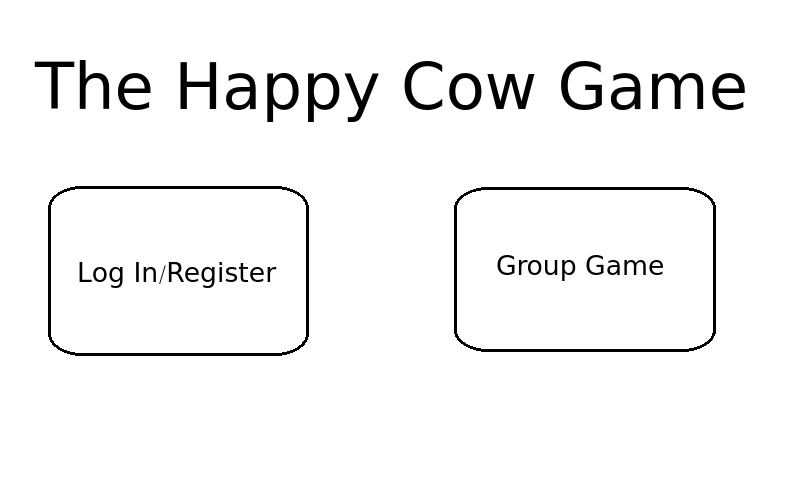
\includegraphics[width=4in]{Images/app3/pages-1-index}}
\end{center}
This is the index page, the first page a user sees. It gives the options of loging in and registering, or creating a group game. A group game will only be possible in a later phase of development.

\subsubsection{Login Page}
\begin{center}
	\fbox{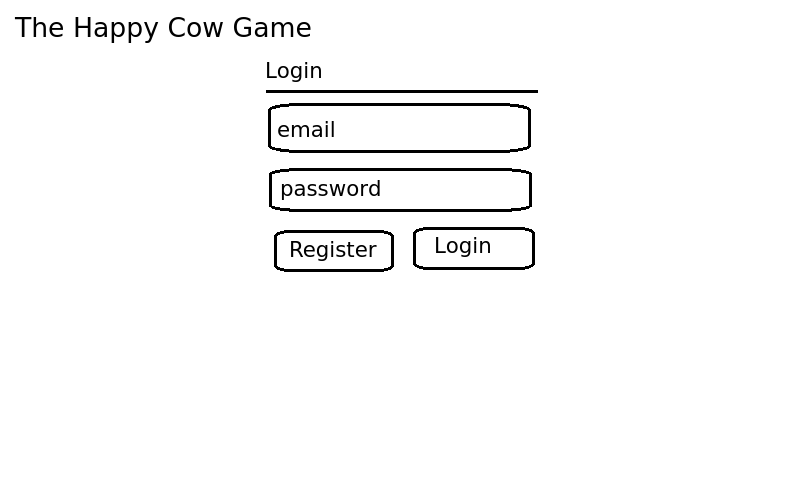
\includegraphics[width=4in]{Images/app3/pages-2-login}}
\end{center}
The login page allows a user to authenticate themselves with their email and password. There is also an option to register, if the user is new to the site.

\subsubsection{Register Page}
\begin{center}
	\fbox{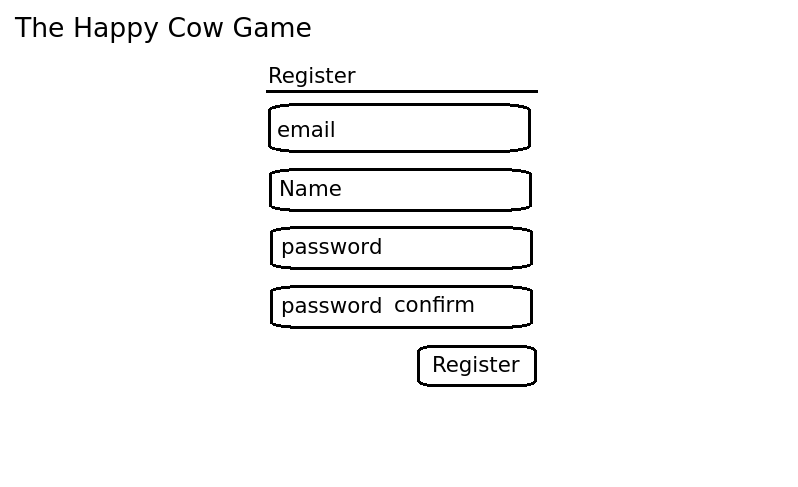
\includegraphics[width=4in]{Images/app3/pages-3-register}}
\end{center}
The register page is designed to look similar to the login page, but with a few more feilds. This means that when choosing to register instead of logging in, the page updates and simply asks for a name and confirmation of the password as well.

\subsubsection{Games List Page}
\begin{center}
	\fbox{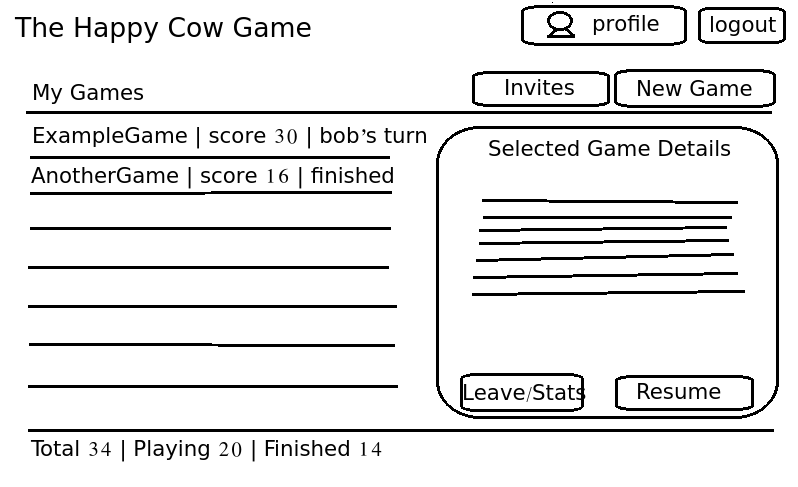
\includegraphics[width=4in]{Images/app3/pages-4-games}}
\end{center}
The game list page is the entry point for games, and other options available to a user. From here a user can see different games they are involved in, and a few details of each. Options allow a user to resume a game, or leave it if they don't want to play anymore. Other menu buttons allow a user to begin a game and view their profile.

\subsubsection{Profile Page}
\begin{center}
	\fbox{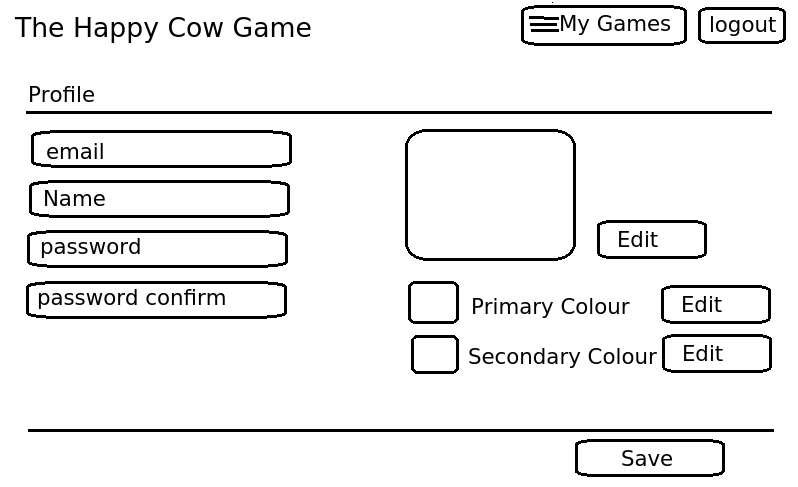
\includegraphics[width=4in]{Images/app3/pages-5-profile}}
\end{center}
This page allows a user to view and edit their personal details. The details needed to register are on the right. When updating a password or email, a confirmation email will be sent. The details on the right are to do with how users are represented in a game.

\subsubsection{Game Setup Page}
\begin{center}
	\fbox{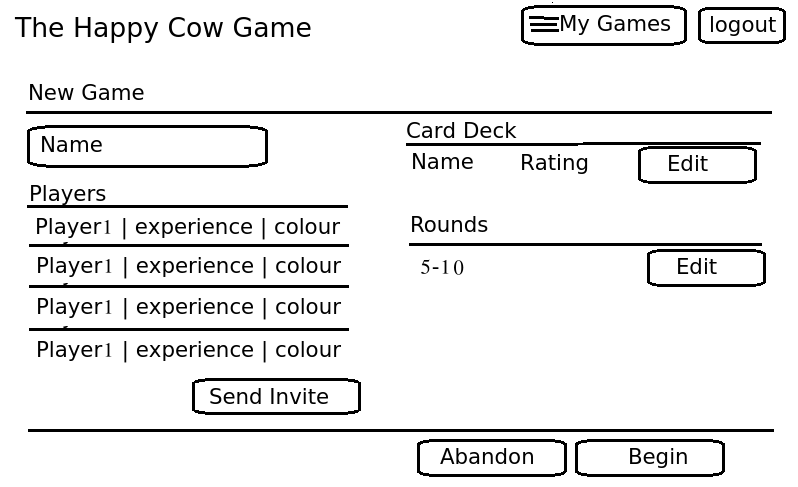
\includegraphics[width=4in]{Images/app3/pages-6-new}}
\end{center}
This page allows a user to create a new game. They can choose a name, a deck of cards to use, and the length of the game. They can also send invites to other players. At first these will be a link allowing a player to join a game themselves, but later if time allows, will be a message within the game.

For players who aren't creators but are joining a game, the edit buttons will not be available. The only action possible will be 'Join' or 'Leave'.

\subsubsection{Play Game Page}
This page is far more detailed than those above, and is described in the following section. When players resume a game, this page is loaded and guides them through the various changes and phases of a game.


\subsection{Game Play User Interface}
The game play page is a single page application. That means it does not require a page load to update data on the page. Instead this is done behind the scenes via Ajax requests to the server. The methods to do this are discussed in the next section. Here the layout of this SPA is considered.

\subsubsection{Menu}
Basic controls of the game appear in a menu at the top of the screen. These include:
\begin{itemize}
	\item A \textbf{Main Menu} with options to return to the game list page, or log out. More features can be added to this list if time allows, such as view statistics of the game.
	\item An overview of the \textbf{Score}. This shows the authenticated player's score, and when clicked, ranks the players in order of score.
	\item \textbf{Messages} will not be implemented in the core functionality.
	\item The \textbf{Round} button shows the current round, and also allows players to see the review phases of previous rounds.
	\item The \textbf{Phases} buttons show the current phase, but give players the ability to visit previous phases. The current phase may have a series of actions. Yet if the current phase is the cards phase, a player can still see the state of the board in the movement phase, but cannot perform any actions.
	\item The \textbf{Active Player} button shows the player whose turn it currently is. A drop down also shows the current order of play, as this changes from round to round.
\end{itemize}
\begin{center}
	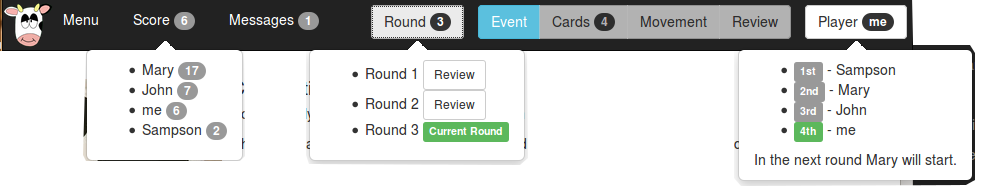
\includegraphics[width=5in]{Images/app3/ui-menu}
\end{center}

\subsubsection{Cow Information}
This section of the user interface, like the menu, is always visible. It shows the state of the cow.
\begin{center}
	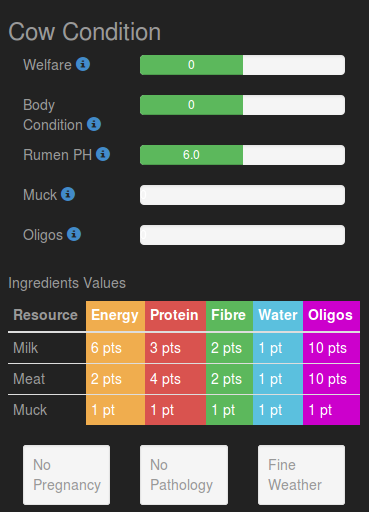
\includegraphics[width=2.5in]{Images/app3/ui-cow-info}
\end{center}

Five markers are shown: Welfare, Body Condition, Rumen PH, Muck and Oligos. These are updated as the game progresses and give an overview of various statistics.

The points that ingredients score are also shown, as these can change. This gives players an idea of what ingredients to include in their rations, and where to try and get their rations absorbed.

Finally there are a few events that remain from turn to turn. These are shown at the bottom and updated as events change.

\subsubsection{Event Phase}
The first of the four phases is the Event Phase. An event will usually have consequences for a player, but these happen later in the game play. The only action available to a player is to review the phase and move on to the cards phase. An example event is shown below.
\begin{center}
	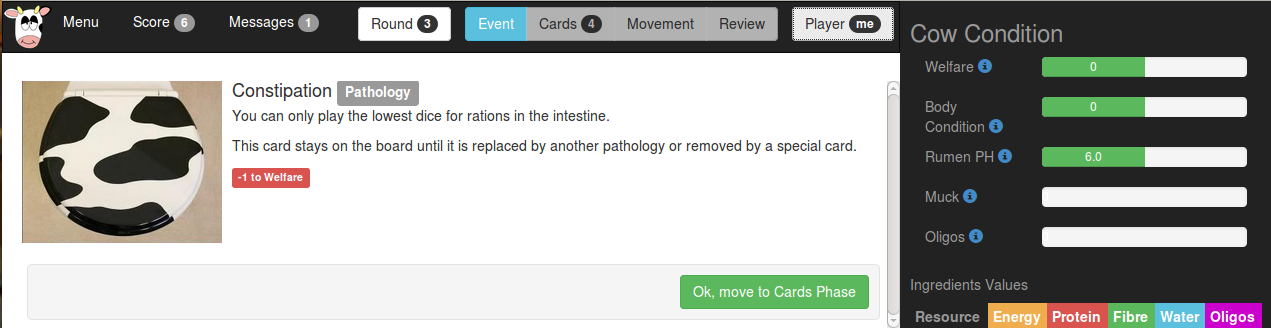
\includegraphics[width=\textwidth]{Images/app3/ui-phase-event}
\end{center}

\subsubsection{Cards Phase}
The second phase is the cards phase. Players receive two new cards at the start of this phase, and can see their deck in a scrollable list of cards. Actions are shown below the cards, and for more details a player can click on a card.

Below the list of cards a player can view their existing rations, and create a new ration if they have at least one ingredient and do not already have four rations. By clicking the 'Use' button below an ingredient, the ingredient appears in the list of ingredients ready to be made into a ration. When ready the player can click to create the ration.
\begin{center}
	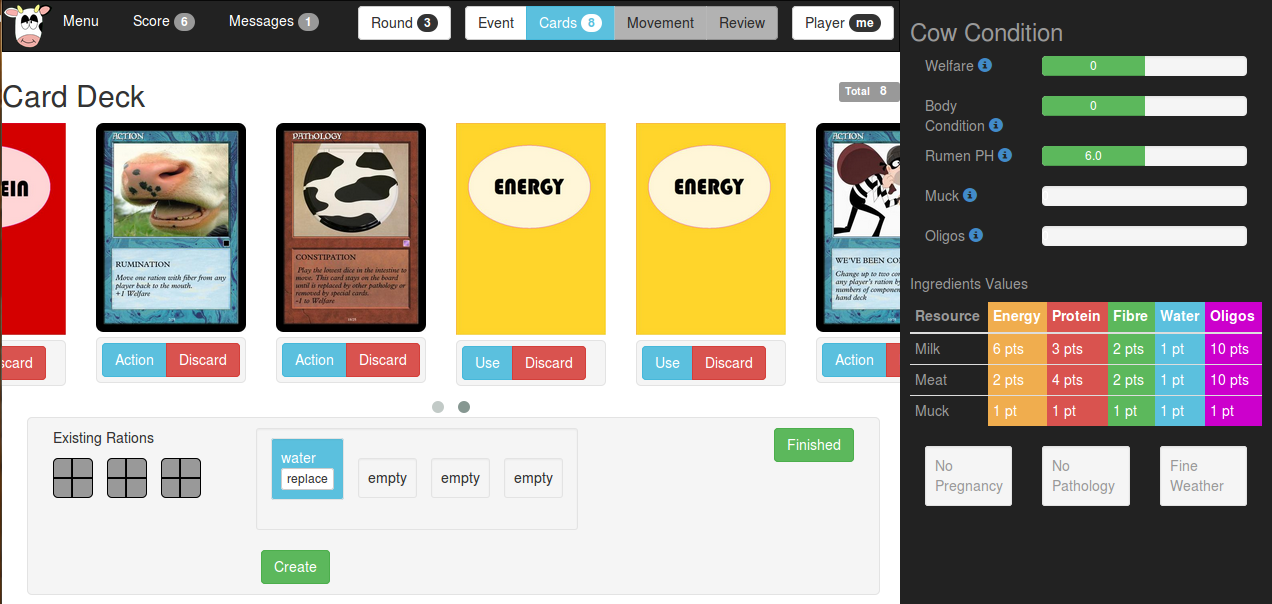
\includegraphics[width=\textwidth]{Images/app3/ui-phase-cards}
\end{center}

Only one ration can be made per player, per round. A modal is displayed to confirm that the user wants to create a ration with the selected ingredients. If they are sure, they confirm their choice and the corresponding ingredient cards in their hand are removed.
\begin{center}
	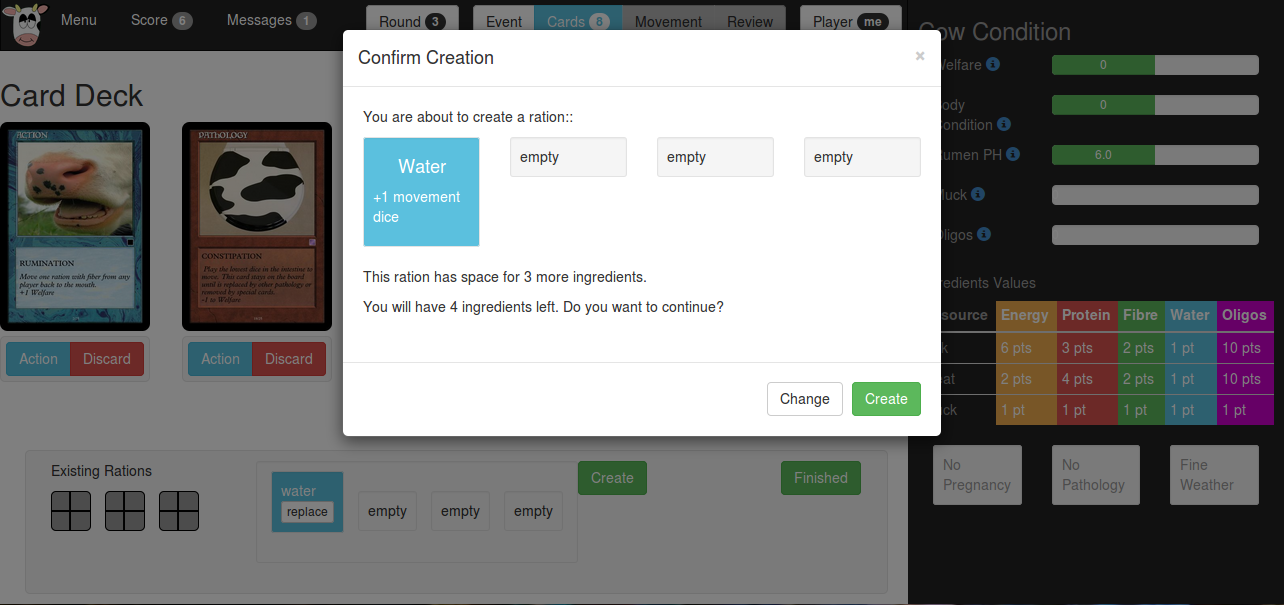
\includegraphics[width=\textwidth]{Images/app3/ui-phase-cards-create}
\end{center}

The player can continue to perform actions on action cards, or discard cards. When they are ready to move on, they end the phase.

\subsubsection{Movement Phase}
The third phase is the movement phase. In this phase the player must select a ration to move, and then select a movement amount offered by the dice. So there are 3 actions within this phase:
\begin{itemize}
	\item Select a ration. The player can click on the rations in the bottom control bar, and the board will move so that the ration is shown in the centre. They then confirm their choice of ration to move.
	\item Select a movement amount. Only once a ration is selected are the movement amounts for that ration calculated and shown. The player can then select the different dice, and the squares where the ration can move are highlighted.
	\item Move the ration. By clicking on one of the highlighted squares, the player confirms their choice of movement. As a player clicks on a square, the ration is shown to 'hop' to that square. The player must keep clicking until all the movements are used up.
\end{itemize}
Once all the movements are used up for the selected ration, the player's movement phase is automatically over.
\begin{center}
	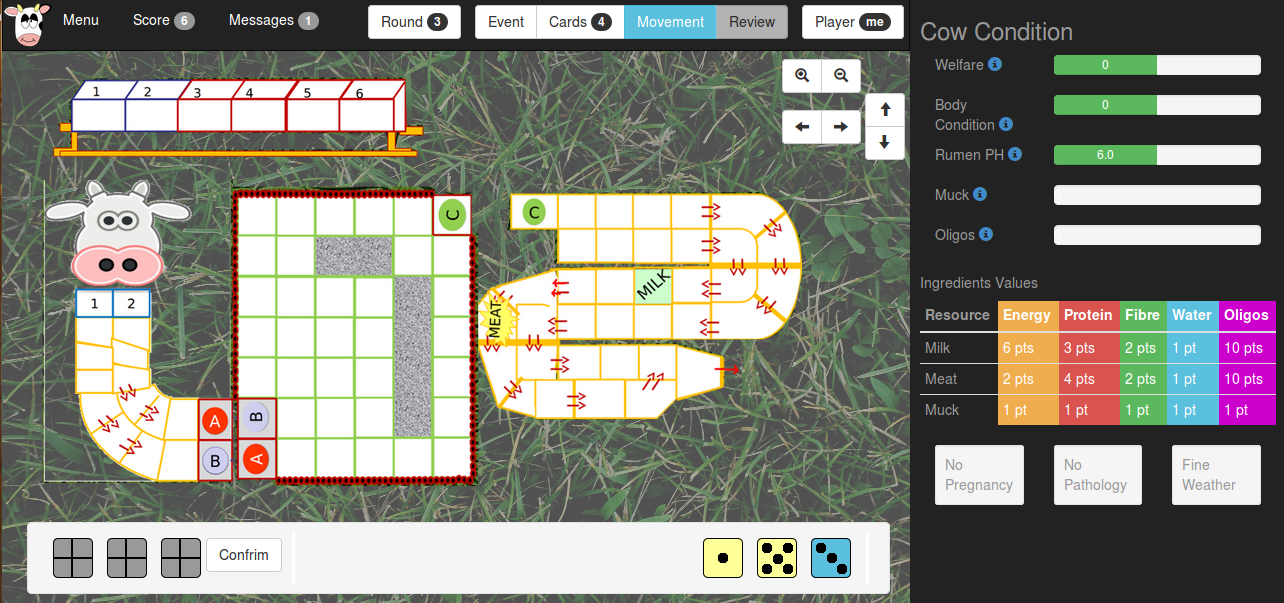
\includegraphics[width=\textwidth]{Images/app3/ui-phase-move}
\end{center}

\subsubsection{Review Phase}
The fourth and final phase is the review phase. No actions are available, but to confirm that they are ready to move on. The player is shown a list of actions that have happened this round, and the current level of points for the round.
\begin{center}
	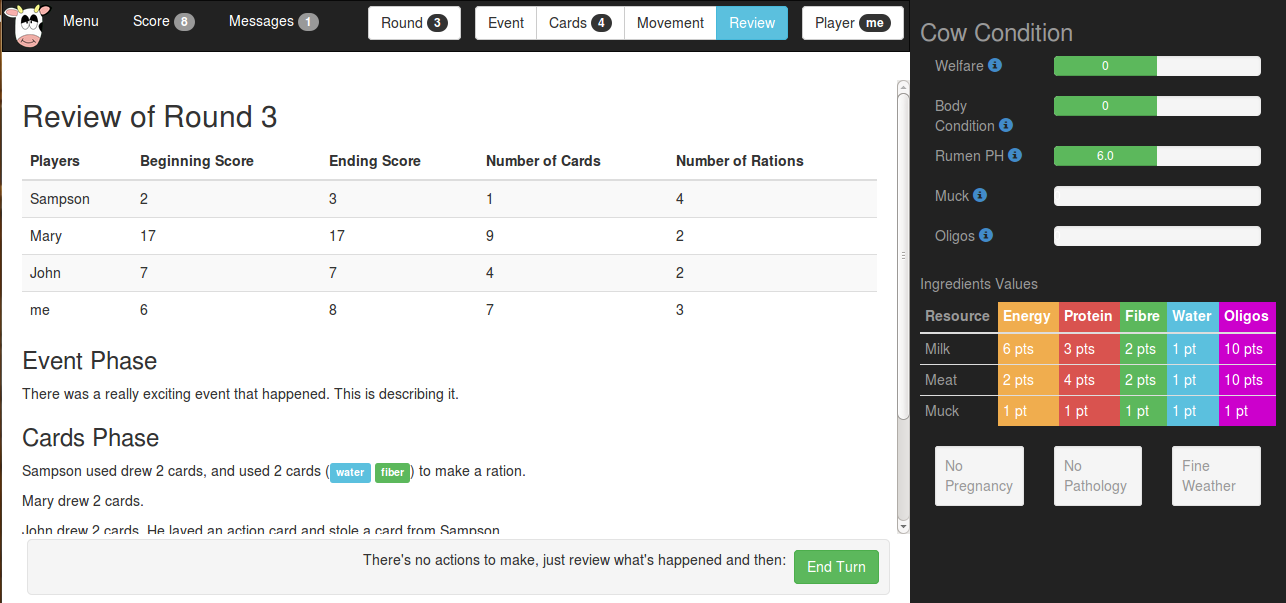
\includegraphics[width=\textwidth]{Images/app3/ui-phase-review}
\end{center}

When all the players indicate they are ready to move on, the next round begins.

\subsection{AngularJS}
This section delves into the different components that make up the game play page. AngularJS uses controllers and services to separate concerns. Controllers perform logic on data that is represented in the Document Object Model (DOM), and therefore each 'functional area' of a page (called the 'view' in Angular terms), should be operated by a separate controller \cite{AngularBook}, page 28. Services, on the other hand, can be created when needed to perform actions within the controllers. Examples are routing and data storage.

\subsubsection{Controllers}
The controllers needed to display and update data within the game play page are listed below.
\begin{enumerate}
	\item \textbf{MenuController} This is a parent controller for the operations of the menu bar at the top of the page.
	\begin{enumerate}
		\item \textbf{MenuViewController} This controller manages a drop down menu with options to leave the game play area, logout, ect.
		\item \textbf{ScoreViewController} This controller manages a drop down menu showing the players in order of score. It also displays the score and position of the player. Further information about scores throughout the game, and how to score points, can be accessed.
		\item \textbf{RoundViewController} This controller manages a drop down menu showing the number of rounds played, and the current round. It offers the option to review previous rounds, allowing users to access the review information from previous rounds.
		\item \textbf{PhaseViewController} This controller shows the current phase by highlighting the current phase and updating the phase on user clicks.
		\item \textbf{Player View Controller} This controller shows the active player, and manages a drop down menu showing the player playing order.
	\end{enumerate}

	\item \textbf{CowController}
This is a parent controller for the cow information display, to the right of the page.
	\begin{enumerate}
		\item \textbf{CowStatsController} This controller manages the progress bars which show the welfare, body condition, rumen PH, muck and oligos markers. These need to be updated automatically as the game progresses.
		\item \textbf{IngredientValueController} This controller manages the table of ingredient values, updating their values as events cause changes.
		\item \textbf{CowEventsController} This controller manages the Pregnancy, Diseases and Weather areas that show changes to cow behaviour caused by events.
	\end{enumerate}

	\item \textbf{PhaseController}
This is a parent controller for the display of the main area of the board. It is changed as players view different phases using the PhaseViewController.
	\begin{enumerate}
		\item \textbf{EventController} This controller manages the template showing the event of the round.
		\item \textbf{CardsController} This controller is a parent of those which manage the actions related to cards.
		\begin{enumerate}
			\item \textbf{CardDeckController} This controller manages actions of cards, and also displays modals with more details of the cards and their causes.
			\item \textbf{CreateRationController} This controller manages uses of ingredients and displays rations as they are created. A modal is provided to review a ration to confirm creation.
			\item \textbf{ExistingRationsController} This controller shows the existing rations, and manages pop-ups showing their position. If a ration is created, it updates to show it.
		\end{enumerate}
		\item \textbf{MovementController} This controller is a parent of those which control movement of rations.
		\begin{enumerate}
			\item \textbf{BoardController} This controller manages the zooming, scrolling, and automatic changes of the board as rations are selected.
			\item \textbf{RationMovementController} Once a ration is selected, this controller manages the actions needed to highlight it, show it's possible movements and update it's position.
			\item \textbf{RationSelectionController} This controller manages the selection of controllers and dice to decide it's movement. Rations and dice need to be disabled once one is chosen.
		\end{enumerate}
		\item \textbf{ReviewController} This controller manages the template showing the actions that have happened during the round.
	\end{enumerate}
	\item \textbf{AlertsController} This controller manages the alerts created by user actions, displaying and deleting them.
\end{enumerate}

\subsubsection{Services}
Currently known services needed are:
\begin{itemize}
	\item An \textbf{\$resource} service. This extends the \$http service and is especially designed for use with a RESTful API. It will perform requests to the server. Many of the controllers will need to do this to perform actions players have requested, and update the page with the responses.
	\item An \textbf{\$animate} service. This helps angular perform basic animations on elements within the page.
	\item An \textbf{Alerts} service. This will allow any controller to create alerts. The AlertsController will be integrated to display alerts that are generated by this service.
	\item A \textbf{LocalStorageModule} service (\url{https://github.com/grevory/angular-local-storage}). This will be used during development to store data instead of sending it to the server. Once the prototype is complete, this will be replaced by the \textbf{\$http} service.
\end{itemize}

%==============================================================================
\section{Detailed Design Sections}
Some areas of the game will be straight forward, and simply involve implementing the API and client side structure above. Other sections require some more thought, however. The aim of this section is to identify and briefly consider these sections.

\subsection{Drawing and Moving Rations}
Once created, a ration has a place on the game board. This has to be both persisted in a database, and represented to the user. To do this, a table of positions is stored, the same list exists for every game instance. Positions need to know where they should appear on the game board. For this reason they have a centre position, indicated by an x and y value. These values correspond to a position on the game board, measured from the top left.

A ration has a record of it's position. It always has a position. If it is absorbed or leaves the cow, it scores points and is then removed. A ration can therefore, use it's position's coordinates to decide where it appears on the board.

\begin{center}
	\fbox{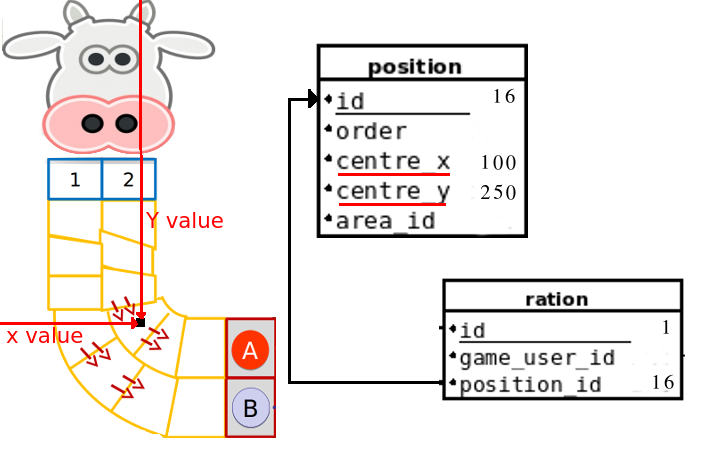
\includegraphics[width=5in]{Images/app3/detail-1}}
\end{center}

As well as x and y coordinates, positions also have a concept of 'next positions'. This means that a position knows which positions a ration can move to from it, and vice versa. This creates a data structure called a graph, where nodes (positions) are connected by one-way relations. When moving a ration, it is therefore possible to look up which positions can be moved to from the current position. This is possible using the server API \textbf{/positions/[id]/graph/[number]} where [id] is the current position, and [number] is the value of the dice.

\begin{center}
	\fbox{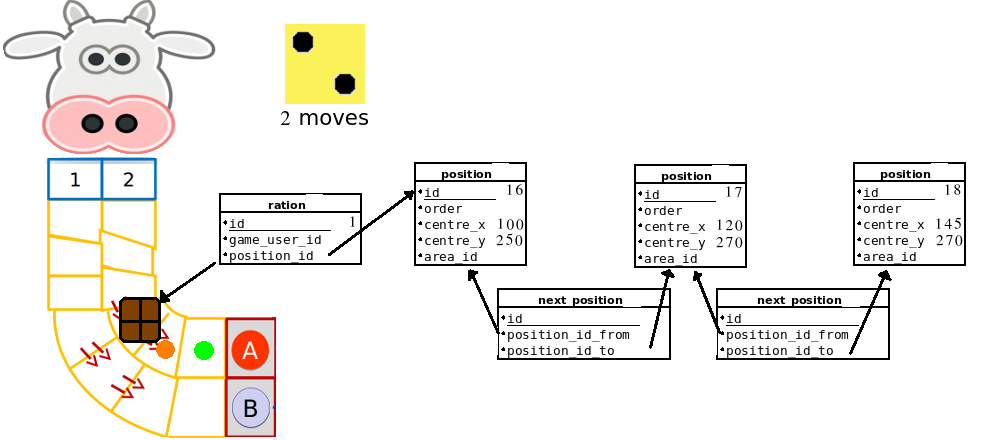
\includegraphics[width=5in]{Images/app3/detail-2}}
\end{center}

In this example, the ration can move 2 spaces. Because the ration is on a bend, the only relations between positions are forwards, down the oesophagus. The ration must move through the first position, so it is marked in orange, but can only finish in the second position, so it is marked in green. These colours help players to see where their rations are allowed to go as they select different dice, and think about which movement to use.

The final challenge is animating the movement. A ration moves one position at a time, as the player must choose which position to move to if there is more than one option. The animation can be done using the coordinates of the two positions, the current position of the ration and the new position of the ration. The difference of the coordinates for x and y is determined, and then divided by 10. The ration is then moved by this amount every 50 mili-seconds. After half a second the animation will be complete.

\subsection{Ordering Positions}
To be able to order rations based on their progress through the cow digestive system, positions need an order. When rations are displayed in the cards or movement phase, they can then be ordered by the order of their positions, without having to work out an order using the graph of positions, which would be computationally expensive. In the oesophagus and intestines the order is fairly straight forward, and can be determined based on the distance from the entry point. In the rumen, the order will be across, so the numbers increase as they go down and to the right.

\begin{center}
	\fbox{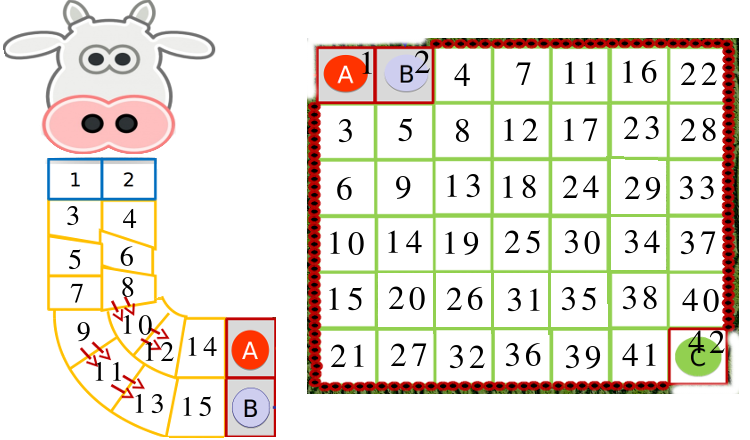
\includegraphics[width=4in]{Images/app3/detail-3}}
\end{center}

As well as providing an order of rations that can be used for display, and resolving some actions, an order to positions as an added advantage when it comes to pushing rations. Rations can be pushed by other rations with more fiber. To work out the direction the attacked ration should be pushed in, the order of positions can be used. If the order of the position the pushing ration came in is less than the order of the current position, then the attacked ration must be pushed to a position with a larger order.

\begin{center}
	\fbox{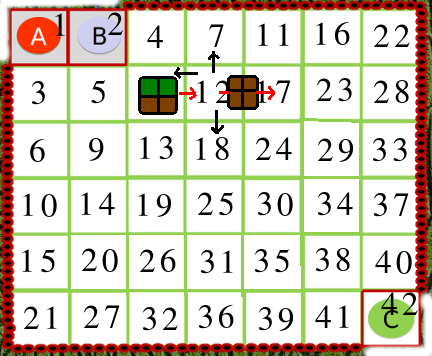
\includegraphics[width=4in]{Images/app3/detail-4}}
\end{center}

In the example above a ration in position ordered 8 is moving to position ordered 12 and has fiber, so can push a ration already on that position. But which direction should the ration be pushed? It is obvious to us, but not with a graph data structure. Instead of comparing coordinates, which could become very complicated in the oesophagus or intestines, the order can be used. There are four possible positions: 7, 8, 17 and 18. The pushing ration is from the second lowest position, so it pushes to the second highest position. If it came from the lowest position it would push to the highest position, and vice versa.

\subsection{Invites}
When a player creates a game, he will want other players to join in. This is done through invitations. One player has control over the creation of a game in order to avoid conflicts when setting a game up.

Initially, to invite another player to a game, the creator of the game will have to send an invitation as a URL to a page via some form of social media. That will allow the player they contact to login, and visit the same game creation page. The player joining will see the name and choice of cards for the game, as well as the list of players who have already joined the game, but they will only be able to perform two actions: join or leave. If they join, a \textbf{game\_users} record is created for that player. If they then decide to leave the game, that record is deleted.

Messages are an extra feature of the project, to be implemented in a later phase. An invitation will be a special form of message that appears in a list of invites for each user. It is essentially an in-game message of the type above that directs a player to the game setup page. They then join or leave as described above.
